\begin{figure}
\centering
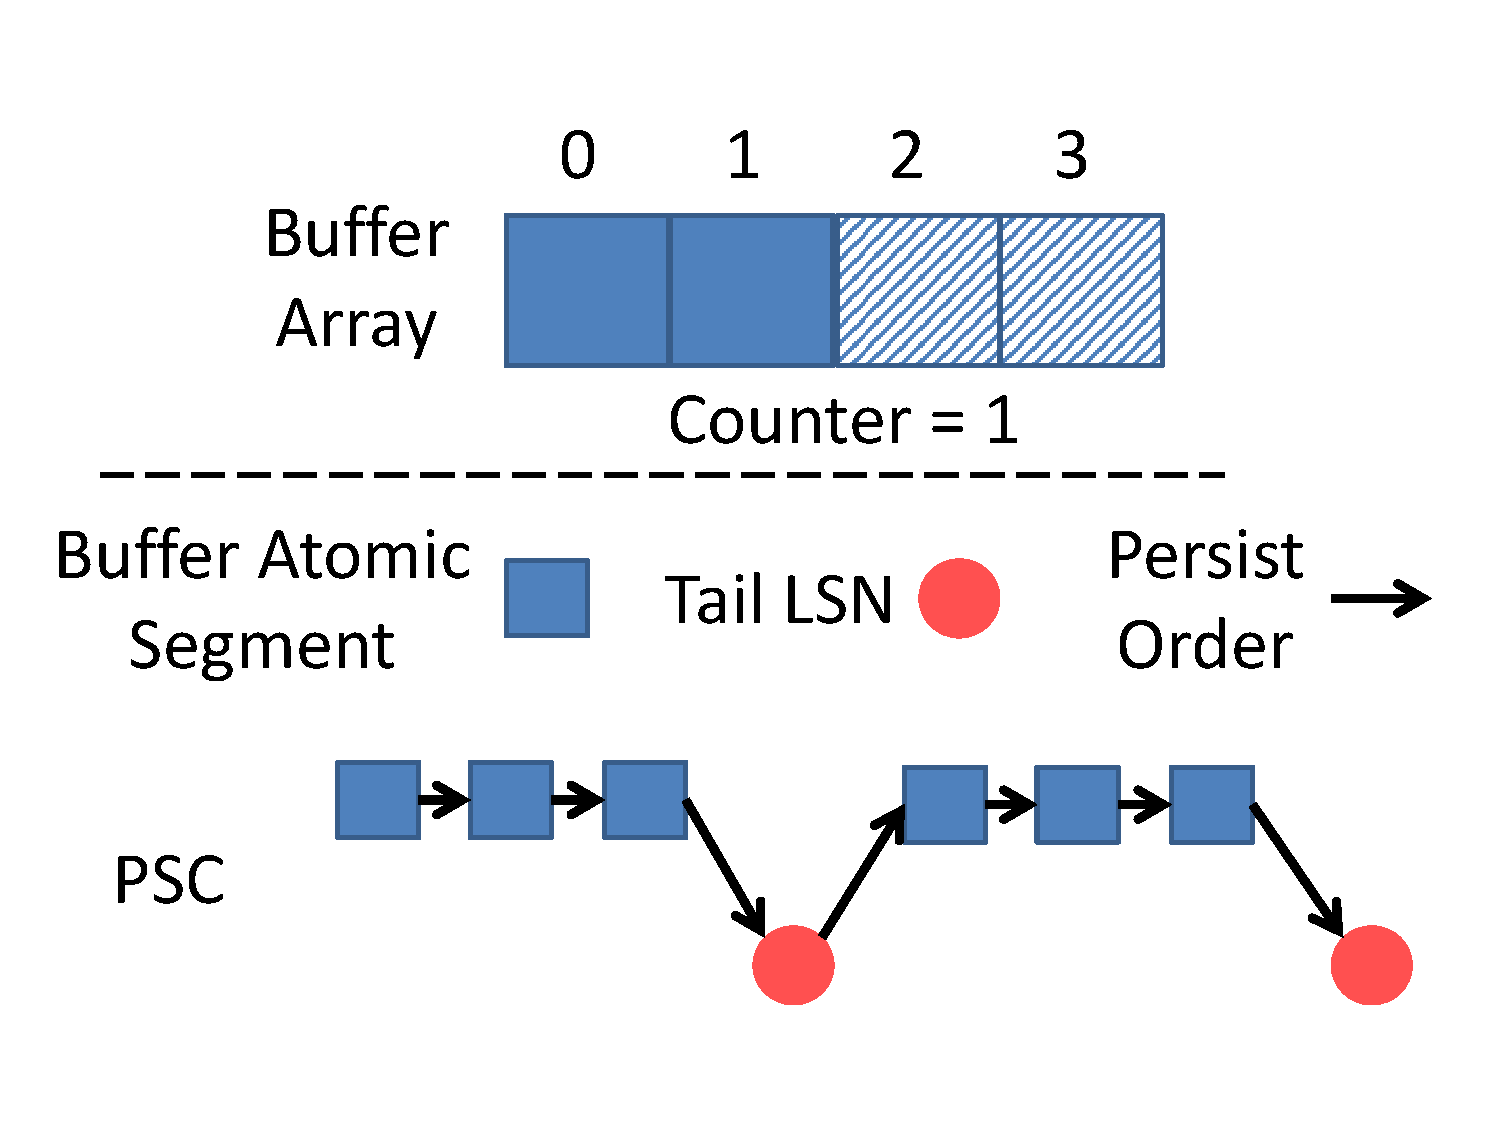
\includegraphics[width=\textwidth]{PMC_patterns/buffer.pdf}
\caption{Persistent buffer. The persistent buffer constists of a persistent array and counter (top).  The array holds persistent data.  The persistent counter marks the greatest persistent slot.  Persisting to the buffer under PSC places depdencies between writing buffer data and updating the counter, as well between persisting the counter and the next buffer persist, forming a chain (bottom).  This occurs both for single threaded and multithreaded use.}
\label{figure::buffer}
\end{figure}
